%%%%%%%%%%%%%%%%%%%%%%%%%%%%%%%%%%%%%%%%%
% Modelo Latex para pôster do SBrT'24
%
% v1: Diego da Silva de Medeiros - IFSC
% v2: Leonardo Lira Ramalho - UFPA
%%%%%%%%%%%%%%%%%%%%%%%%%%%%%%%%%%%%%%%%%

%----------------------------------------------------------------------------------------
%	PACKAGES AND OTHER DOCUMENT CONFIGURATIONS
%----------------------------------------------------------------------------------------

\documentclass[a0,portrait]{a0poster}

\usepackage{multicol} % This is so we can have multiple columns of text side-by-side
\columnsep=100pt % This is the amount of white space between the columns in the poster
\columnseprule=3pt % This is the thickness of the black line between the columns in the poster
\usepackage{fancybox}
\usepackage[svgnames]{xcolor} % Specify colors by their 'svgnames', for a full list of all colors available see here: http://www.latextemplates.com/svgnames-colors

\usepackage{pdfpages}
\usepackage{color}
\usepackage{colortbl}
\usepackage[cmex10]{amsmath}
\usepackage{amssymb}
\usepackage{soul}
%\usepackage{mathtools}
\usepackage[normalem]{ulem}
%\graphicspath{{fig/}}
%\usepackage{soul}
\usepackage{booktabs}
\usepackage{color}
\usepackage{placeins}
\usepackage{upgreek}
\usepackage[utf8]{inputenc}
\usepackage{bm,bbm}
\usepackage[export]{adjustbox}
\usepackage[sort&compress]{natbib}

%\usepackage{times} % Use the times font
%\usepackage{palatino} % Uncomment to use the Palatino font
\usepackage{epstopdf}
\usepackage{graphicx} % Required for including images
%\graphicspath{{figures/}} % Location of the graphics files
\usepackage[font=small,labelfont=bf]{caption} % Required for specifying captions to tables and figures
\usepackage{amsfonts, amsmath, amsthm, amssymb} % For math fonts, symbols and environments
\usepackage{wrapfig} % Allows wrapping text around tables and figures
\usepackage[framemethod=TikZ]{mdframed}
\usepackage{titlesec} % Modify titles
%\usepackage{fontspec}
%\setmainfont{Calibri}
\newcommand{\ds}{\displaystyle}
\newcommand {\bo}[1]{\textbf{#1}}
\newcommand{\pa}[1]{\left({#1}\right)}
\newcommand{\co}[1]{\left[{#1}\right]}
\newcommand{\ch}[1]{\left\{{#1}\right\}}

\titleformat{\section}{\color{white}\normalfont\Large\bfseries}{\color{white}\thesection}{1em}{\colorbox{SteelBlue}}{}

\setlength{\columnseprule}{0pt}
\mdfdefinestyle{MyFrame}{%
	linecolor=SteelBlue,
	outerlinewidth=2pt,
	roundcorner=50pt,
	innertopmargin=\baselineskip,
	innerbottommargin=\baselineskip,
	innerrightmargin=20pt,
	innerleftmargin=20pt,
	backgroundcolor=white!50!white}
%\input{figconfig}
%\titleformat{command}[shape]{format}{label}{sep}{be %fore-code}{after-code}
\begin{document}
\begin{mdframed}[style=MyFrame]
%----------------------------------------------------------------------------------------
%	POSTER HEADER 
%----------------------------------------------------------------------------------------

% The header is divided into two boxes:
% The first is 75% wide and houses the title, subtitle, names, university/organization and contact information
% The second is 25% wide and houses a logo for your university/organization or a photo of you
% The widths of these boxes can be easily edited to accommodate your content as you see fit
\begin{minipage}[b]{0.33\linewidth}
\raggedright
\includegraphics[width=12cm,valign=t]{NZSA-logo-words-e1505785105112-1.png}
\end{minipage}
%
\begin{minipage}[b]{0.33\linewidth}
\centering
\hfill
%\includegraphics[width=50cm,valign=t]{img_sbrt24_poster.pdf}
\end{minipage}
% 
\begin{minipage}[b]{0.33\linewidth}
\raggedleft
\includegraphics[width=11cm,valign=t]{Logo Offshore Standard Landscape Reversed RGB.png}
\end{minipage}\\

\vspace{3cm}
\begin{minipage}[h]{0.98\linewidth}
\centering \huge \color{SteelBlue} \textbf{Ordinal Pattern Analysis for Early Bearing Fault Detection and Classification in Rotating Machinery -- First Results} \color{Black}\\ % Title
\Large \textbf{Rasika Dilhani\textsuperscript{1}, and Alejandro C.\ Frery\textsuperscript{2}}\\ % Author(s)
\normalsize School of Mathematics and Statistics, Victoria University of Wellington, New Zealand \\ %[-0.5cm] % University/organization
rasidilhani@gmail.com\textsuperscript{1} and alejandro.frery@vuw.ac.nz\textsuperscript{2}\\
\end{minipage}
\vspace{0.5cm} % A bit of extra whitespace between the header and poster content

%----------------------------------------------------------------------------------------

\begin{multicols}{2} % This is how many columns your poster will be broken into, a portrait poster is generally split into 2 columns

%-----------------------------------------------------------------------------

%	INTRODUCTION
%----------------------------------------------------------------------------------------

\section{Introduction}

Ordinal Patterns are transformations that encode the sorting characteristics of values in $\mathbbm R^D$ into $D!$ symbols.

They were proposed by Bandt \& Pompe in 2002, and have proven their adequacy at extracting valuable information about the system that produces the data.

One of the possible encodings is the set of indexes that sort the $D$ values in non-decreasing order, for example:
$$
(4.2, 5.1, 7.1, 3.9, 8.6) \longmapsto (2, 3, 4, 1, 5) \longmapsto \beth \text{ (one of }5!=120 \text{ symbols)}.
$$
A time series $\bm x = (x_1,x_2,\dots,x_{D+n-1})$ can be transformed into a sequence of symbols $\bm \pi=(\pi_1,\pi_2,\dots,\pi_n)$ where $\pi_i=\pi_i(x_i,x_{i+1},\dots, x_{i+D-1})$; $D$ is called the ``embedding dimension,'' and usually ranges between $3$ and $6$.
Then, we compute $\bm h =(p_1,p_2,\dots,p_{D!})$ the histogram of $\bm \pi$, and obtain two descriptors.
The first is the Shannon entropy, a measure of the system's disorder:
\begin{equation}
    H[p]=-\frac{1}{\log D!}\sum_{i=1}^{D!}{p_i \log p_i}
    \label{eq:ShannonEntropy}
\end{equation}
with the convention that terms in the summation for which $p_i=0$ are null. This quantity is bounded in the unit interval. 
It is zero when $p_i=1$ for some $i$ (and, thus, all other bins are zero), and one when $p_i=1/D!$ for every $i$ (the uniform probability function); it is also called ``permutation entropy.''

%In Shannon entropy, complexity can be inferred from the level of unpredictability in the system. 
%In permutation entropy, complexity measures capture patterns in ordinal sequences. 
%Other measure statistical complexity refine this by combining entropy and additional features of the system’s structure.

Another descriptor, the complexity $C$ quantifies the balance between randomness and structure in a system. It evaluates how much order or pattern there is in the system while taking into account the inherent unpredictability. In addition, $C$ distinguishes different levels of periodicity and other important properties, providing insights into the dynamic behavior of the system.

An arbitrary time series analyzed with embedding dimension $D$ and mapped on histograms of $D!$ bins can produce any set of points $(H, C)$ that make up the entropy–complexity plane. 

\begin{minipage}{\columnwidth}
    \includegraphics[width=\linewidth]{AllSystems.pdf}
    
   \textbf{Fig:1} The $H\times C$ plane for $D=6$ with examples of time series and their points. FROM: \citet{chagas2022white}
\end{minipage}

Recently, \citet{REY2024115481} obtained the asymptotic variance of the permutation entropy: 
Asymptotic variance in the
$H \times C$ 
plane along with the confidence intervals for their Shannon entropy is defined as follows. Sample Shannon entropy 
$(\widehat{H}(x)$ 
with sample asymptotic variance 
$(s^2(x)$ 
is calculated to obtain the asymptotic confidence interval at level $1 − \alpha$

\begin{equation}
    \widehat{H}[\alpha]-Z_{\alpha/2} \frac{S(X)}{\sqrt{n-D}},  \widehat{H}[\alpha]+Z_{\alpha/2} \frac{S(X)}{\sqrt{n-D}}
    \label{eq:Asymptotic variance}
\end{equation}
where $X$ is the time series with length $n$, and the ordinal patterns were computed with embedding dimension $D$.  
 
This result enhances the use of the Entropy-Complexity plane in time series analysis.

\section{Data}\label{section1}

The data were obtained from the Bearing Data Center and the seeded fault test data at the Case Western Reserve University, School of Engineering. 
The dataset includes ball bearing test data for normal bearings, as well as single-point defects on the drive end and fan end. 
Data were collected at rates of 12,000 and 48,000 data points per second for the drive-end bearing tests and at 12,000 data points per second for the fan-end
bearing tests. Each file includes motor rotational speed, drive-end vibration data, and fan-end vibration data. The variable names in each file
indicate the following:
\begin{itemize}
        \item DE - drive end accelerometer data
        \item FE - fan end accelerometer data
	\item BA - base accelerometer data
	\item time - time series data
	\item RPM - rpm during testing
\end{itemize}
	
For ease of use, the data were categorized as Normal Baseline Data, 12k Drive End Bearing Fault Data, 48k Drive End Bearing Fault Data, and Fan
End Bearing Fault Data. The normal baseline data include four motor load levels: 0, 1, 2, and 3, with approximate motor speeds provided in RPM
(1797, 1772, 1750, and 1730). The 12k Drive End, 48k Drive End, and 12k Fan End bearing data follow the same motor load levels and speeds. This
research aims to identify faulty machines using the time series of their measured features.

% ACF Those plots conveyed almost no information
%\vspace{1cm}
%\hspace{1cm}
%\begin{minipage}{\columnwidth}
%    \includegraphics[width=0.9\columnwidth]{group_plot_normal.pdf}
%\end{minipage}
%\hspace{1cm}
%\vspace{1cm} %\\\vspace{-10cm}

%\hspace{1cm}
%\begin{minipage}{\columnwidth}
%    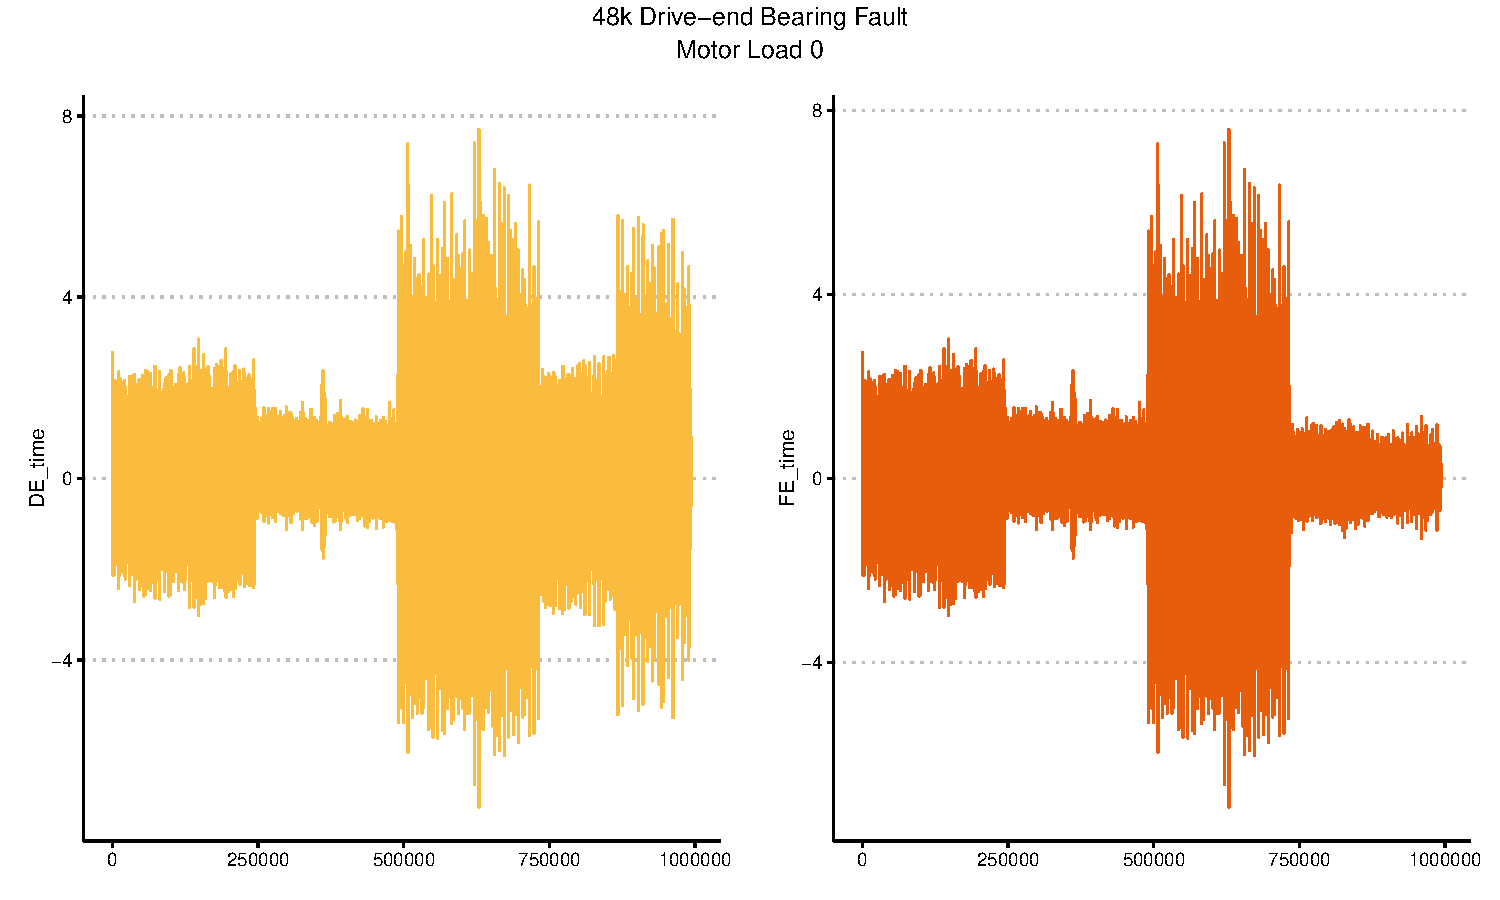
\includegraphics[width=0.9\columnwidth]{group_plot_.pdf}
%\end{minipage}
%\hspace{1cm}

\section{Methodology}\label{section2}

With an emphasis on common fault types like ball, outer race, and inner race defects, this study investigates the application of ordinal pattern analysis for the early detection and classification of bearing faults. The goal of this study is to locate malfunctioning machinery. We use ordinal patterns to analyze the two time series in each data file. Based on the ordinal structure of the segments, we introduce distance as a metric of similarity. This metric can be used to identify malfunctioning machines with certain embedding dimensions. We demonstrate that embedding dimensions ranging from 3 to 6 effectively separate defective machines by using permutation entropy for rolling bearing fault diagnosis. The results of embedding dimension 4 with normal base line and 48k drive end time series data are presented in this article. White noise is found close to the upper and lower limits. With the graph below, it is evident. The results are analyzed using the complexity plane, which confirms that dimension 4 produces the best results to date. Time series data were first examined, and the StatOrdPatt package was then used to analyze the data using the methodology outlined by Rey et al. (2024). The entropy permutation entropy was then computed taking into account the ordinal pattern's probability distribution. To identify the malfunctioning machines, the entropy complexity level was taken into consideration based on the entropy of each time series data set.

\section{Results}\label{section3}
The embedding dimension 4 results for normal base line and 48k drive are considered to set up this analysis. Figure 2 shows the DE, and FE time series for engine loads 0, 1, 2 and 3. The graph is clear and it can be seen that it is failure time series data is about time series. However, it is difficult to separate the exact machine type and other characteristics of the data. The main idea of this research work is to identify perturbation machines using the various time series data given above. 

\begin{minipage}{\columnwidth}
    \includegraphics[width=0.9\columnwidth]{confidence_interval.pdf}
    
 \textbf{Fig:2} Entropies with their confidence intervals in the $H\times C$ plane.
\end{minipage}

\section{Conclusion and Future Work} \label{section4}

Permutation entropy guarantees the separation of error machines. With this experimental result, we can see that the embedding dimension 4 result in separate error machines. We see that the machines form clusters, but also that they have individual signatures. The points of the time series in the $H \times C$ plane as well as the confidence intervals for their Shannon entropies are taken into account.

This research will be expanded to analyze embedding dimensions from 3 to 6, offering deeper insights into the dynamics of ordinal time series. Additionally, we will leverage the remaining dataset for a comprehensive analysis. A key focus will be on exploring feature selection techniques based on cluster and variability analyses tailored for ordinal multi-class classification problems, advancing the understanding of these complex systems.

Notably, much of the existing research has concentrated on univariate time series, despite the prevalence of multivariate scenarios in real-world applications. To address this gap, our study extends to multivariate time series analysis. By employing confidence interval-based approaches and asymptotic variance as tools for classification, we have achieved promising results that underline the novelty of our work. These findings highlight the potential of our methods to set a benchmark, encouraging to explore multivariate contexts with similar frameworks.

\section*{Acknowledgements}
\bibliographystyle{agsm}
\bibliography{BearingFaultDiagnosis}

%---------------------------------------------------
-------------------------------------
\end{multicols}
\begin{center}
\color{SteelBlue}{NZSA Conference, Victoria University of Wellington, December 2024}
\end{center}
\end{mdframed}
\end{document}

General comments:
* Make the text more concise. Do not repeat what has already been said
* Include the confidence intervals for the entropy
* Make the plots fonts serif to match the text
* Align the VUW logo to the right (I did this in the document I edited and synchronized)
* Emphasize the novelty and relevance of using the confidence intervals
